\documentclass{standalone}
\usepackage{tikz}
\usepackage{pgfplots}
\pgfplotsset{compat=1.18}

\begin{document}
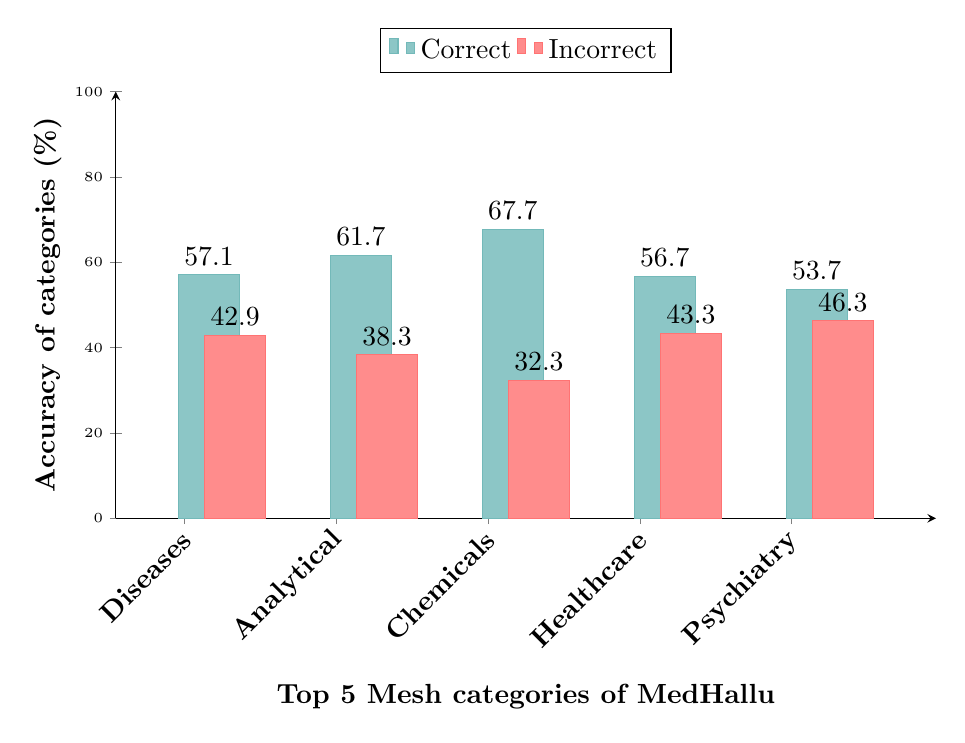
\begin{tikzpicture}
\tiny
\begin{axis}[
    width=12cm,
    height=7cm,
    ybar=-40pt,    % Reduced from 8pt to bring bars closer
    bar width=22pt,
    ylabel={\normalsize\textbf{Accuracy of categories (\%)}},
    xlabel={\normalsize\textbf{Top 5 Mesh categories of MedHallu}},
    xlabel style={yshift=-1em}, 
    symbolic x coords={D1,D2,A1,A2,C1,C2,H1,H2,P1,P2},
    xtick={D1,A1,C1,H1,P1},
    xticklabels={\normalsize\textbf{Diseases}, \normalsize\textbf{Analytical}, \normalsize\textbf{Chemicals}, \normalsize\textbf{Healthcare}, \normalsize\textbf{Psychiatry}},
    xticklabel style={
        rotate=45,           % Rotates labels 45 degrees
        anchor=east,         % Aligns the labels properly
        yshift=-0.5em        % Adjusts vertical position
    },
    legend style={
        at={(0.5,1.15)},
        anchor=north,
        legend columns=2,
        font=\normalsize
    },
    ymin=0,
    ymax=100,   % Changed to a percentage scale
    axis lines=left,
    clip=false,
    enlarge x limits=0.1,  % Reduced side margins
    nodes near coords,
    nodes near coords style={font=\normalsize},
    every node near coord/.append style={yshift=1pt}
]

% Calculated percentages (rounded to one decimal place):
% Diseases: Correct: 148/259*100 ≈ 57.1, Incorrect: 111/259*100 ≈ 42.9
% Analytical: Correct: 124/201*100 ≈ 61.7, Incorrect: 77/201*100 ≈ 38.3
% Chemicals: Correct: 107/158*100 ≈ 67.7, Incorrect: 51/158*100 ≈ 32.3
% Healthcare: Correct: 55/97*100 ≈ 56.7, Incorrect: 42/97*100 ≈ 43.3
% Psychiatry: Correct: 36/67*100 ≈ 53.7, Incorrect: 31/67*100 ≈ 46.3

\addplot[fill=teal!45!white, draw=teal!55!white] coordinates {
    (D1,57.1) (A1,61.7) (C1,67.7) (H1,56.7) (P1,53.7)
}; \addlegendentry{Correct}

\addplot[fill=red!45!white, draw=red!55!white] coordinates {
    (D2,42.9) (A2,38.3) (C2,32.3) (H2,43.3) (P2,46.3)
}; \addlegendentry{Incorrect}

\label{Mesh_class_plot}
\end{axis}
\end{tikzpicture}
\end{document}